\chapter{Quiz R1}
\section{Question 1}
In a DC electrical circuit, a voltage source having an emf of \SI{12}{\volt} is connected to a load having two resistances in series, one resistance is \SI{10}{\ohm} and the other is \SI{5}{\ohm}. Determine the following:
\subsection{a}
Current flowing in the circuit:
\begin{align}
    V & = IR                \\
    I & = \frac{V}{R}       \\
    I & = \frac{12}{15}     \\
    I & = \SI{0.8}{\ampere}
\end{align}
\subsection{b}
Voltage across the \SI{10}{\ohm} resistor:
\begin{align}
    V & = IR            \\
    V & = 0.8\times 10  \\
    V & = \SI{8}{\volt}
\end{align}
\subsection{c}
Voltage across the \SI{5}{\ohm} resistor:
\begin{align}
    V & = IR            \\
    V & = 0.8\times 5   \\
    V & = \SI{4}{\volt}
\end{align}
\subsection{d}
Power dissipated in the \SI{10}{\ohm} resistor:
\begin{align}
    P & = IV              \\
    P & = 0.8\times 8     \\
    P & = \SI{6.4}{\watt}
\end{align}
\subsection{e}
Power dissipated in the \SI{5}{\ohm} resistor:
\begin{align}
    P & = IV              \\
    P & = 0.8\times 4     \\
    P & = \SI{3.2}{\watt}
\end{align}
\subsection{f}
Total energy supplied in 10 minutes:
\begin{align}
    E & = Pt                                           \\
    E & = \left(6.4+3.2\right)\left(60\times 10\right) \\
    E & = \SI{5760}{\joule}
\end{align}
\chapter{Quiz 1 - Per Unit Impedance}
\section{Question 1}
The base impedance and base voltage for a given single-phase power system are \SI{10}{\ohm} and \SI{400}{\volt} respectively. Calculate the base kVA and the base current.
\begin{align}
    I_{base} & = \frac{V_{base}}{Z_{base}} = \frac{400}{10} = \SI{40}{\ampere} \\
    S_{base} & = V_{base}\times I_{base} = 400\times 40 = \SI{16}{kVA}
\end{align}
\section{Question 2}
The base current and base voltage of a single-line \SI{345}{\kilo\volt} system are chosen as \SI{3000}{\ampere} and \SI{300}{\kilo\volt}. Determine the pu voltage and the base impedance.
\begin{align}
    V        & = \frac{V_{actual}}{V_{base}} = \frac{345}{300} = \SI{1.15}{pu} \\
    Z_{base} & = \frac{V_{base}}{I_{base}} = \frac{300}{3} = \SI{100}{\ohm}
\end{align}
\section{Question 3}
If the $S$ rating for Question 2 is \SI{1380}{MVA}, calculate the current in amperes and express the current in pu using those base quantities.
\begin{align}
    S & = \SI{1380}{MVA}                                   \\
    V & = \SI{345}{\kilo\volt}                             \\
    I & = \frac{1380\times 10^3}{345} = \SI{4000}{\ampere} \\
    I & = \frac{4000}{3000} = \SI{1.33}{pu}
\end{align}
\section{Question 4}
Express \SI{100}{\ohm} impedance, \SI{60}{\ampere} current and \SI{220}{\volt} voltage as pu quantities using base values obtained in Question 1.
\begin{align}
    Z_{base} & = \SI{10}{\ohm}                   \\
    Z        & = \frac{100}{10} = \SI{10}{pu}    \\
    I_{base} & = \SI{40}{\ampere}                \\
    I        & = \frac{60}{40} = \SI{1.5}{pu}    \\
    V_{base} & = \SI{400}{\volt}                 \\
    V        & = \frac{220}{400} = \SI{0.55}{pu}
\end{align}
\section{Question 5}
Let a \SI{5}{kVA} 400/200 V three-phase transformer be approximately represented by a \SI{2}{\ohm} reactance per phase referred to the low voltage side. Consider the rated values as base quantities and ignore $\sqrt{3}$ in your calculations. Calculate the base current, the base impedance and express the transformer reactance as a per unit quantity.
\begin{align}
    S_{base} & = \SI{5}{kVA}                         \\
    V_{base} & = \SI{200}{V}                         \\
    I_{base} & = \frac{5000}{200} = \SI{25}{\ampere} \\
    Z_{base} & = \frac{200}{25} = \SI{8}{\ohm}       \\
    Z        & = \frac{2}{8} = \SI{0.25}{pu}
\end{align}
\section{Question 6}
Repeat Question 5 expressing the following quantities in terms of the high voltage side: base impedance and per unit impedance.
\begin{align}
    S_{base} & = \SI{5}{kVA}                        \\
    V_{base} & = \SI{400}{V}                        \\
    I_{base} & = \frac{5000}{400} = \SI{12.5}{\ohm} \\
    Z_{base} & = \frac{400}{12.5} = \SI{32}{\ohm}
\end{align}
Note that $Z_{base}$ is now for the HV side. The impedance reflected across the windings of a transformer can be stated as:
\begin{gather}
    Z_{primary} = \left(\frac{N_{primary}}{N_{secondary}}\right)^2\times Z_{secondary}
\end{gather}
where $N$ is the number of winding turns. The pu reactance of a transformer does not change across the windings so pu reactance on the secondary is \SI{0.25}{pu}. Reactance at secondary:
\begin{gather}
    Z_{secondary} = 0.25 \times 32 = \SI{8}{\ohm}
\end{gather}
\section{Question 7}
A three-phase \SI{13}{\kilo\volt} transmission line delivers \SI{8}{MVA} of load. The per phase impedance of the line is $\left(0.01+j0.05\right)$ pu referred to a \SI{13}{\kilo\volt}, \SI{8}{MVA} base. What is the voltage drop across the transmission line?

The per unit base VA and V are the same as the transmission line rating and the transmission line is delivering rated VA to the load so the current flowing must be:
\begin{gather}
    I = \SI{1}{pu}
\end{gather}
Transmission line pu impedance:
\begin{align}
    Z & = \left(0.01+j0.05\right)\, \si{pu}             \\
    Z & = \left(0.01^2+0.05^2\right)^2 = \SI{0.051}{pu}
\end{align}
Potential difference across the transmission line:
\begin{gather}
    V_{line} = I_{pu}Z_{pu} = 1\times 0.051 = \SI{0.051}{pu}
\end{gather}
We know that:
\begin{gather}
    V_{base} = \SI{13}{kV}
\end{gather}
Therefore:
\begin{gather}
    V_{line} = 0.051\times 13000 = \SI{663}{\volt}
\end{gather}
\section{Question 8}
Draw an impedance diagram for the system shown below expressing the results as percentage values to a \SI{10}{MVA}, \SI{66}{kV} base.
\begin{figure}[H]
    \centering
    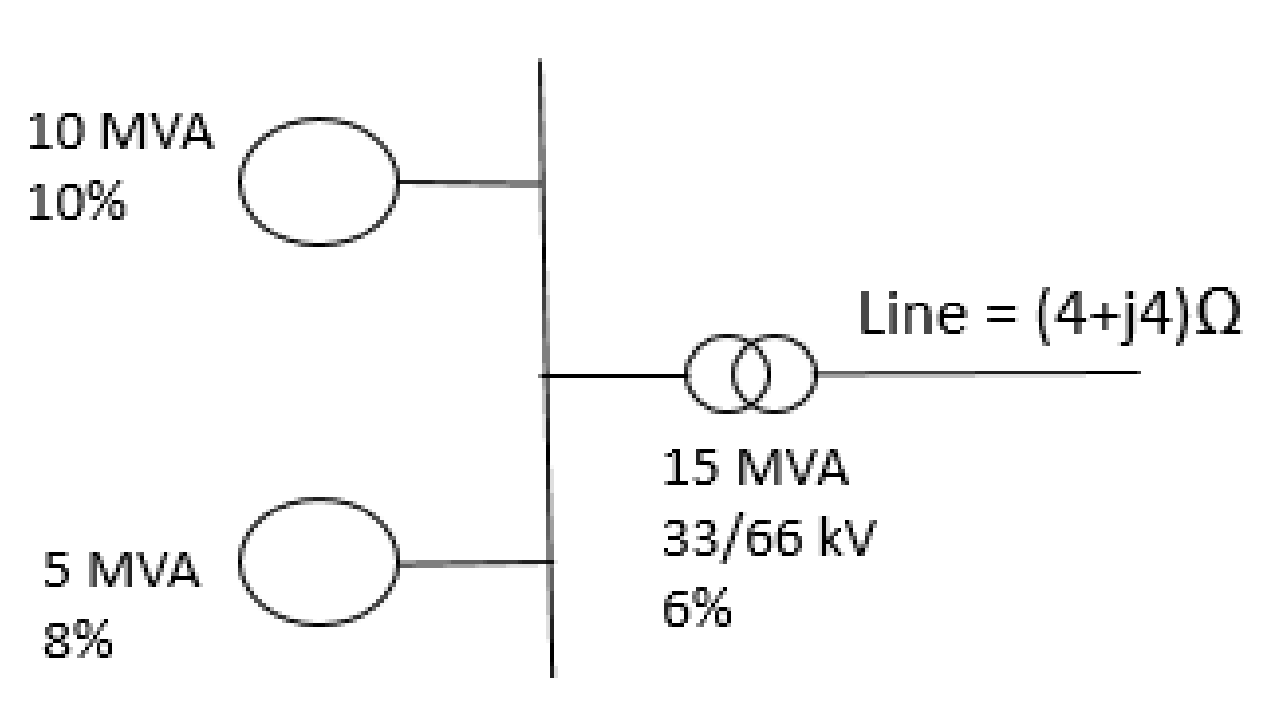
\includegraphics[width = 0.5\textwidth]{img/figure148.png}
    \caption{Quiz 1, Question 8. Diagram.}
\end{figure}
\begin{align}
    S_{base} & = \SI{10}{MVA}                                                 \\
    V_{base} & = \SI{66}{kV}                                                  \\
    I_{base} & = \frac{10\times 10^3}{\sqrt{3}\times 66} = \SI{87.5}{\ampere} \\
    Z_{base} & = \frac{66\times 10^3}{87.5} = \SI{754.3}{\ohm}
\end{align}
Since the two machines are on the \SI{33}{kV} side of the transformer. 10\% is to a \SI{10}{MVA}, \SI{33}{kV} base while the 8\% is to a \SI{5}{MVA}, \SI{33}{kV} base. This may be the manufacturer's rating for per unit purposes. They each have to use their own manufacturer MVA rating for per unit reactance determination or the value would be meaningless. The transformer would be to a \SI{15}{MVA}, \SI{33}{kV} base on the primary side and the transmission line per unit would need to be based on whatever the ohmic per unit value is on the secondary (\SI{66}{kV}) side.

\SI{10}{MVA} machine:
\begin{align}
    S & = \SI{10}{MVA} \\
    V & = \SI{33}{kV}  \\
    Z & = 10\%
\end{align}
Referring to the system base:
\begin{align}
    S & = \frac{10}{10} = \SI{1}{pu}                                       \\
    V & = \frac{33}{66} = \SI{0.5}{pu}                                     \\
    Z & = \frac{10}{10}\times \frac{33^2}{66^2}\times 0.1 = \SI{0.025}{pu}
\end{align}
\SI{5}{MVA} machine:
\begin{align}
    S & = \SI{5}{MVA} \\
    V & = \SI{33}{kV} \\
    Z & = 8\%
\end{align}
Referring to the system base:
\begin{align}
    S & = \frac{5}{10} = \SI{0.5}{pu}                                      \\
    V & = \frac{33}{66} = \SI{0.5}{pu}                                     \\
    Z & = \frac{10}{5}\times \frac{33^2}{66^2} \times 0.08 = \SI{0.04}{pu}
\end{align}
Transformer:
\begin{align}
    S & = \frac{15}{10} = \SI{1.5}{pu} \\
    V & = \frac{0.5}{1} = \SI{0.5}{pu} \\
\end{align}
It is not clear whether the two machines are generators or motors, if the power comes in from the right side and the machines are motors, then the high voltage side would be the primary side? If on transformer HV side:
\begin{align}
    Z & = \frac{10}{15}\times \frac{33^2}{66^2} \times 0.06 = \SI{0.01}{pu}
\end{align}
Line:
\begin{gather}
    Z = \frac{4+j4}{754.3} = 0.005 + j0.005\,\si{pu}
\end{gather}
\section{Question 9}
In a power system, two generators G1 and G2 supply motor load M1, M2 and M3 via transformers T1 and T2 and transmission line L1. Using \SI{100}{MVA}, \SI{33}{kV} base, determine the reactance diagram.
\begin{figure}[H]
    \centering
    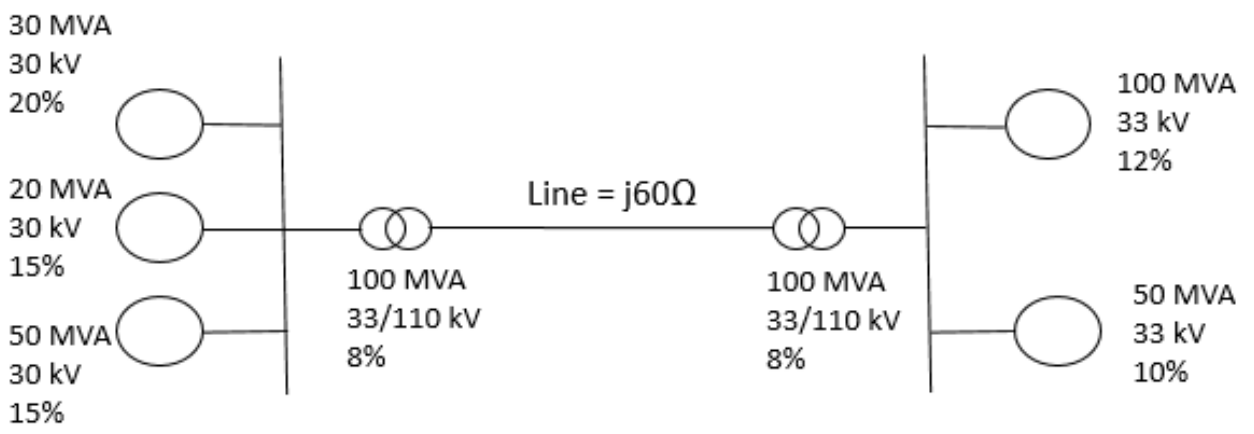
\includegraphics[width = 0.7\textwidth]{img/figure149.png}
    \caption{Quiz 1, Question 9. Diagram.}
\end{figure}
System base:
\begin{align}
    S_{base} & = \SI{100}{MVA}                                               \\
    V_{base} & = \SI{33}{kV}                                                 \\
    I_{base} & = \frac{100\times 10^3}{\sqrt{3}\times 33} = \SI{1749.55}{pu} \\
    Z_{base} & = \frac{33000}{1749.55} = \SI{18.86}{pu}
\end{align}
G1:
\begin{align}
    S & = \frac{100}{100} = \SI{1}{pu} \\
    V & = \frac{33}{33} = \SI{1}{pu}   \\
    Z & = j\SI{0.12}{pu}
\end{align}
G2:
\begin{align}
    S & = \frac{50}{100} = \SI{0.5}{pu}                                     \\
    V & = \frac{33}{33} = \SI{1}{pu}                                        \\
    Z & = \frac{100}{50}\times \frac{33^2}{33^2}\times 0.1 = j\SI{0.12}{pu}
\end{align}
M1:
\begin{align}
    S & = \frac{30}{100} = \SI{0.3}{pu}                                      \\
    V & = \frac{30}{33} = \SI{0.91}{pu}                                      \\
    Z & = \frac{100}{30}\times \frac{30^2}{33^2}\times 0.2 = j\SI{0.551}{pu}
\end{align}
M2:
\begin{align}
    S & = \frac{20}{100} = \SI{0.2}{pu}                                      \\
    V & = \frac{30}{33} = \SI{0.91}{pu}                                      \\
    Z & = \frac{100}{20}\times \frac{30^2}{33^2}\times 0.15 = j\SI{0.62}{pu}
\end{align}
M3:
\begin{align}
    S & = \frac{50}{100} = \SI{0.5}{pu}                                      \\
    V & = \frac{30}{33} = \SI{0.91}{pu}                                      \\
    Z & = \frac{100}{50}\times \frac{30^2}{33^2}\times 0.15 = j\SI{0.25}{pu}
\end{align}
T1 and T2 are already rated at base system values.

Line voltage is \SI{110}{kV}, therefore:
\begin{gather}
    Z = \frac{100}{100}\times \frac{33^2}{110^2}\times \frac{60}{18.86} = j\SI{0.286}{pu}
\end{gather}
\chapter{Quiz 2 - Fundamentals}
\section{Question 1}
A balanced delta-connected load whose branch impedances are 45$\angle$\SI{70}{\degree\ohm}; a three-phase motor that draws a total of \SI{10}{kVA} at 0.65 power factor lagging, and a star load with branch resistance of \SI{10}{\ohm} are all supplied from the same \SI{208}{\volt}, \SI{60}{\hertz} source. Sketch the circuit and then determine the line currents to each three-phase load.
\section{Question 2}
A three-phase, three-wire \SI{500}{\volt}, \SI{60}{\hertz} source supplies a three-phase induction motor; a star connected capacitor bank that draws \SI{2}{kVAR} per phase and a balanced three-phase heater that draws a total of \SI{10}{\kilo\watt}. The induction motor is rated at \SI{75}{hp} and has an efficiency and power factor of 90.5\% and 89.5\% respectively. Draw a one line diagram for the system and then determine:
\begin{enumerate}
    \item The system kW
    \item The system KVAR
    \item The system KVA
\end{enumerate}
\begin{figure}[H]
    \centering
    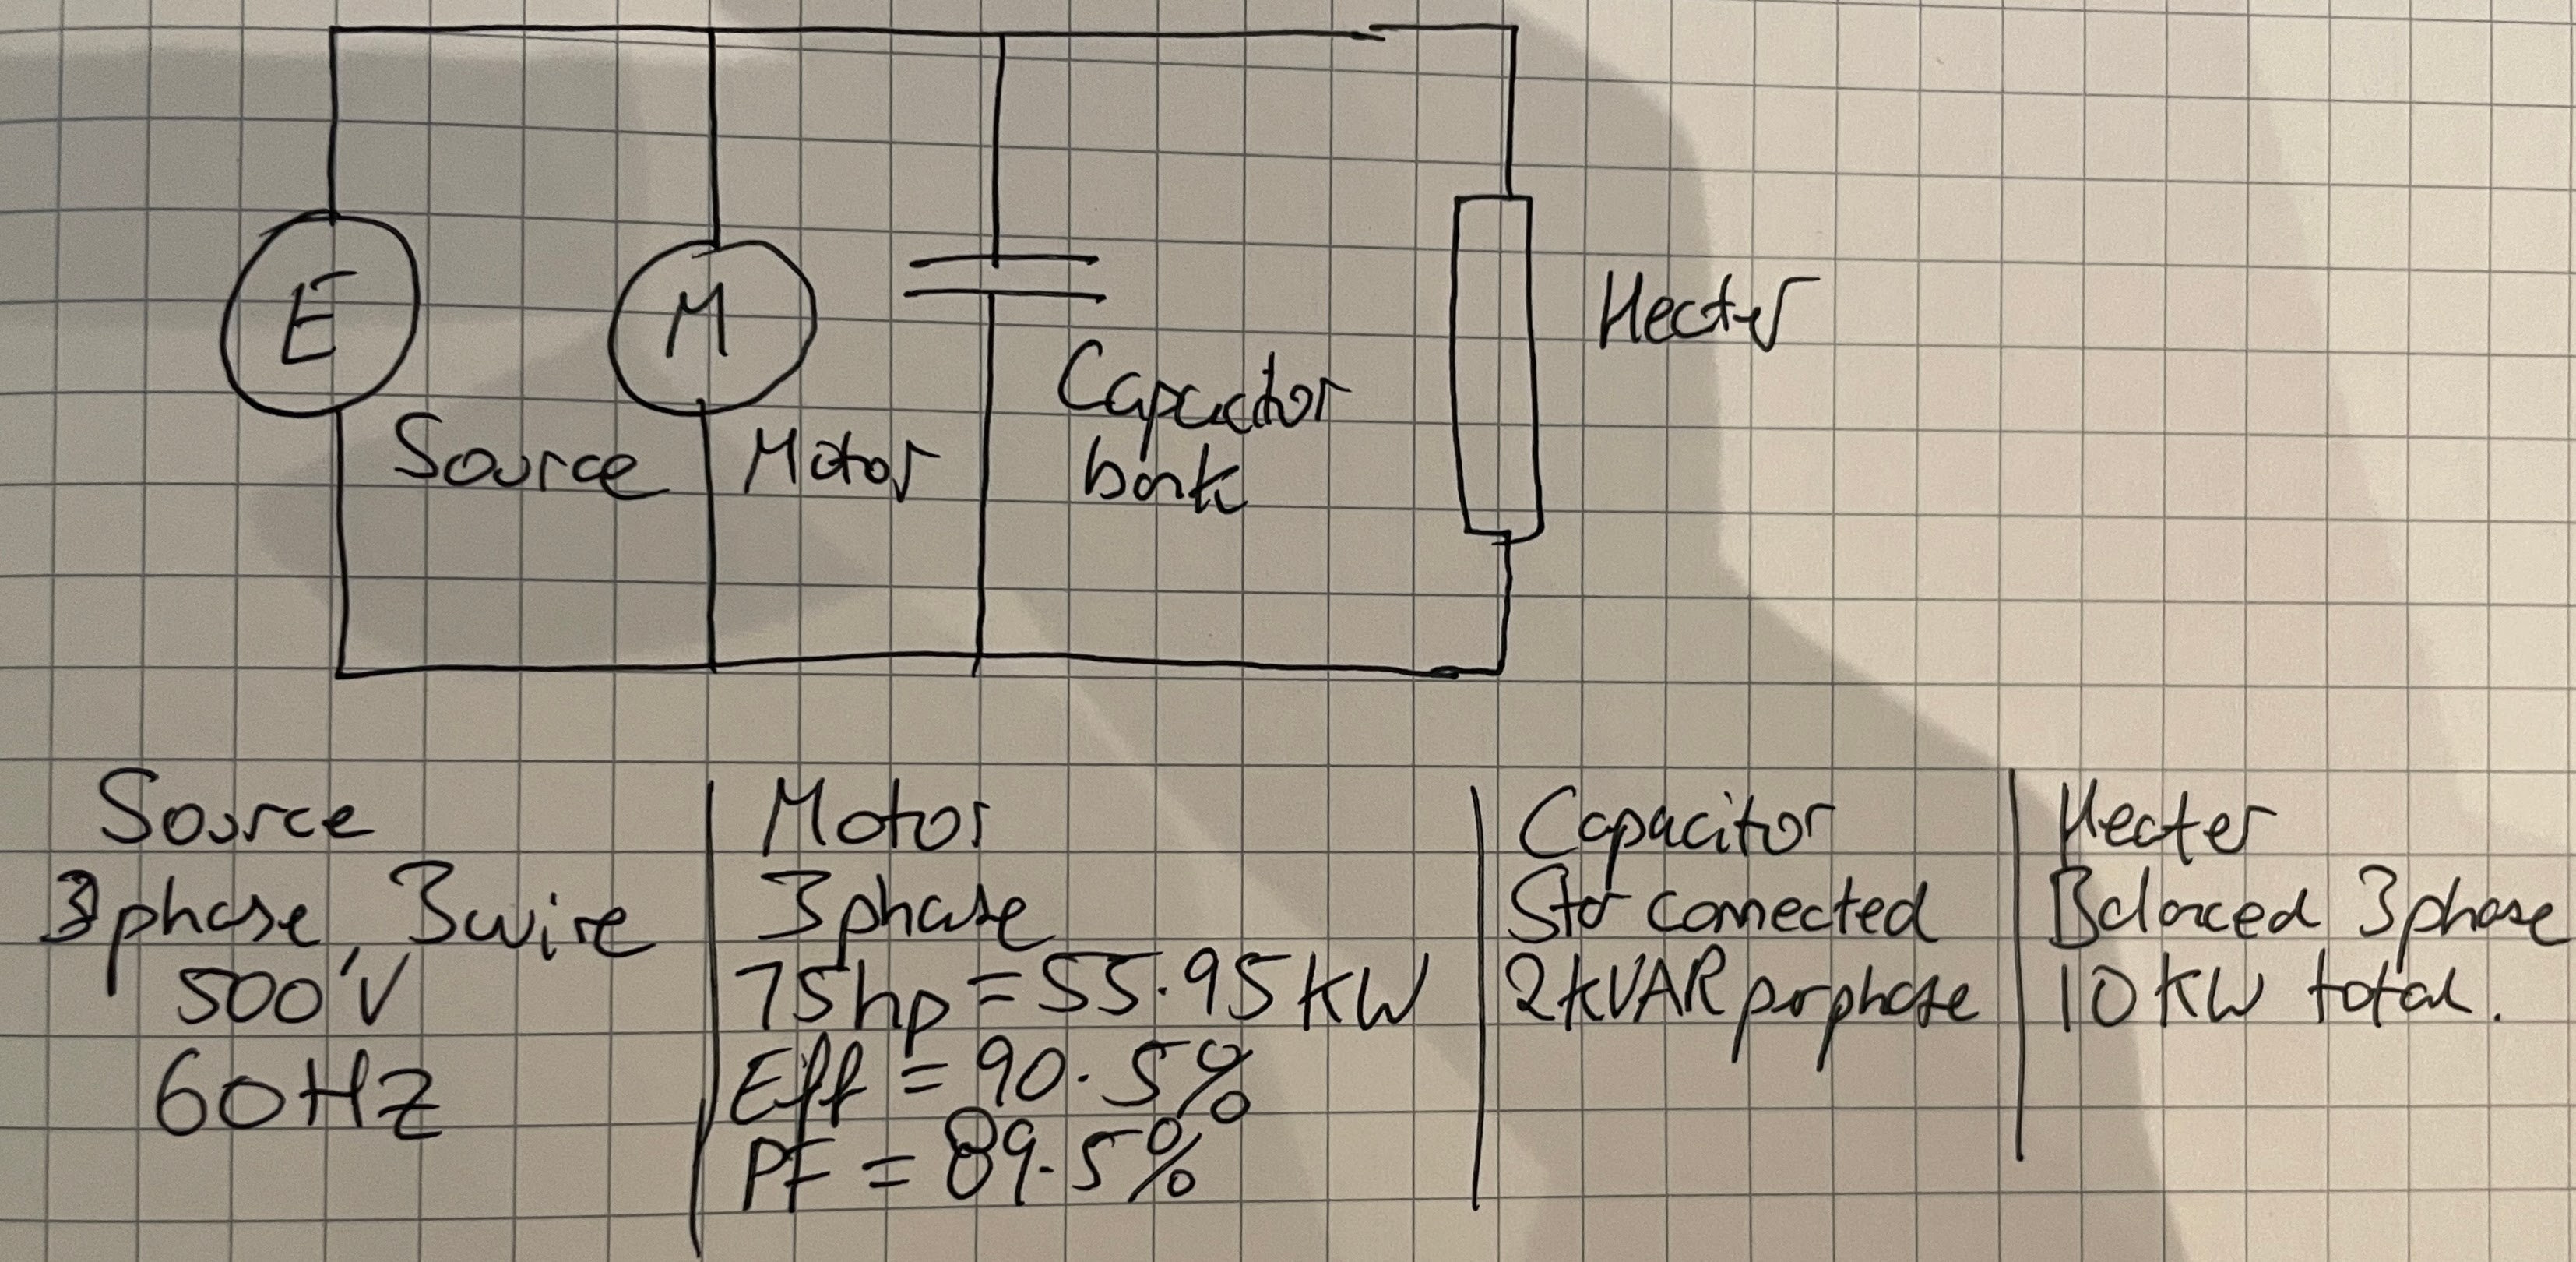
\includegraphics[width = \textwidth]{img/figure151.jpg}
    \caption{Quiz 2, Question 2. Diagram.}
\end{figure}
Power input motor:
\begin{gather}
    P_{m} = \frac{55.95}{0.905} = \SI{61.823}{kW}
\end{gather}
Hence, using power triangle:
\begin{gather}
    \cos\theta = 0.895\\
    \theta = \SI{26.49}{\degree}\\
    Q_{m} = P\tan\theta = 61.823\tan\left(26.49\right) = \SI{30.81}{KVAR}
\end{gather}
Reactive power here is lagging and thus positive.

Capacitor bank is completely reactive, hence:
\begin{align}
    P_{c} & = \SI{0}{kW}    \\
    Q_{c} & = \SI{-6}{kVAR}
\end{align}
This is because it is \SI{2}{kVAR} per phase and it is a three-phase system. Reactive power here is leading and thus negative.

Heater is completely real power.
\begin{align}
    P_h & = \SI{10}{kW}  \\
    Q_h & = \SI{0}{kVAR}
\end{align}
System:
\begin{align}
    P_s & = 61.823+10= \SI{71.823}{kW}                \\
    Q_s & = 30.81-6=\SI{24.81}{kVAR}                  \\
    S_s & = \sqrt{24.81^2+71.823^2} = \SI{75.99}{kVA}
\end{align}
\section{Question 4}
The single line diagram for a three-generator system is shown below. Redraw the diagram to show all values as per unit referred to a \SI{7}{MVA}, \SI{11}{kV} base.
\begin{figure}[H]
    \centering
    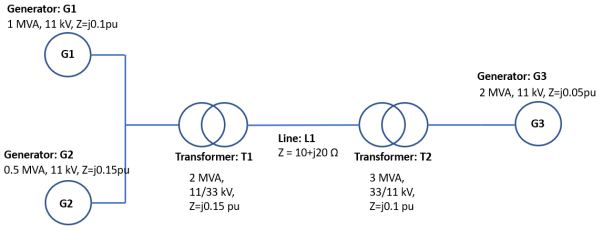
\includegraphics[width = \textwidth]{img/figure153.png}
    \caption{Quiz 2, Question 2. Diagram.}
\end{figure}
Note the different base values used for the line section due to the change in voltage. Since both transformer sides are running at rating, we do not need to change the voltage base in our impedance calculation. Since it is a three-phase system, we include $\sqrt{3}$ in our base value calculations.
\begin{figure}[H]
    \centering
    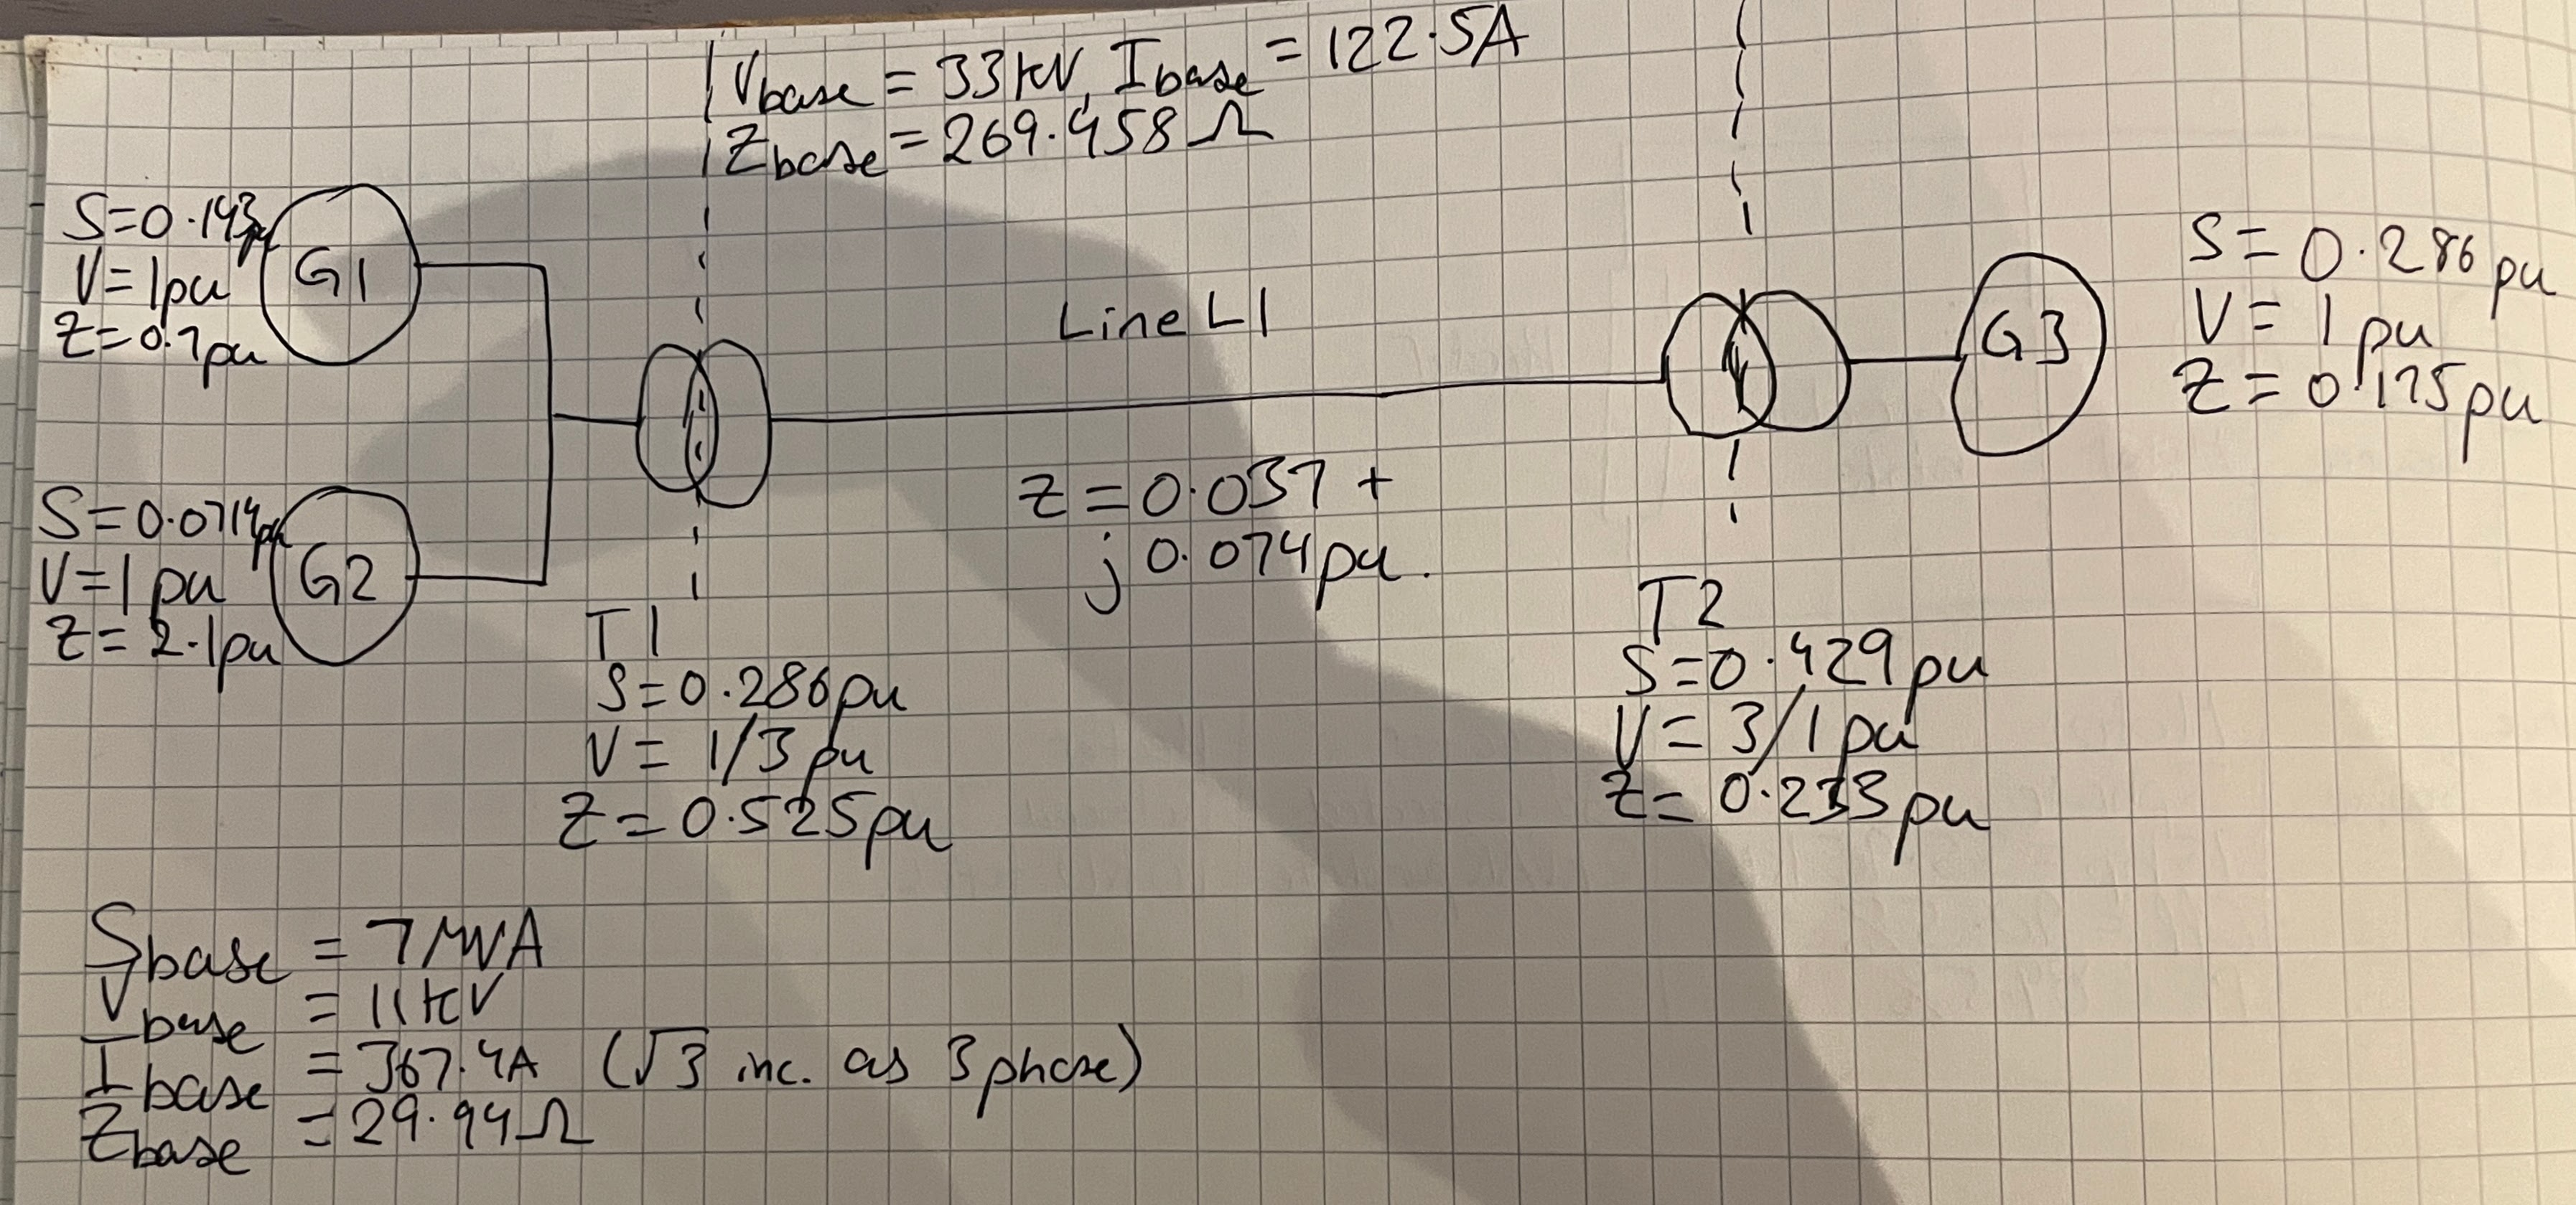
\includegraphics[width = \textwidth]{img/figure152.jpg}
    \caption{Quiz 2, Question 2. Solution Diagram.}
\end{figure}
\chapter{Quiz 3 - Faults}
\section{Question 1}
For the single line diagram shown below and using \SI{480}{\volt}, \SI{20}{kVA} base, determine the `equivalent impedance' of the whole circuit in pu and the current flowing from the generator in pu.
\begin{figure}[H]
    \centering
    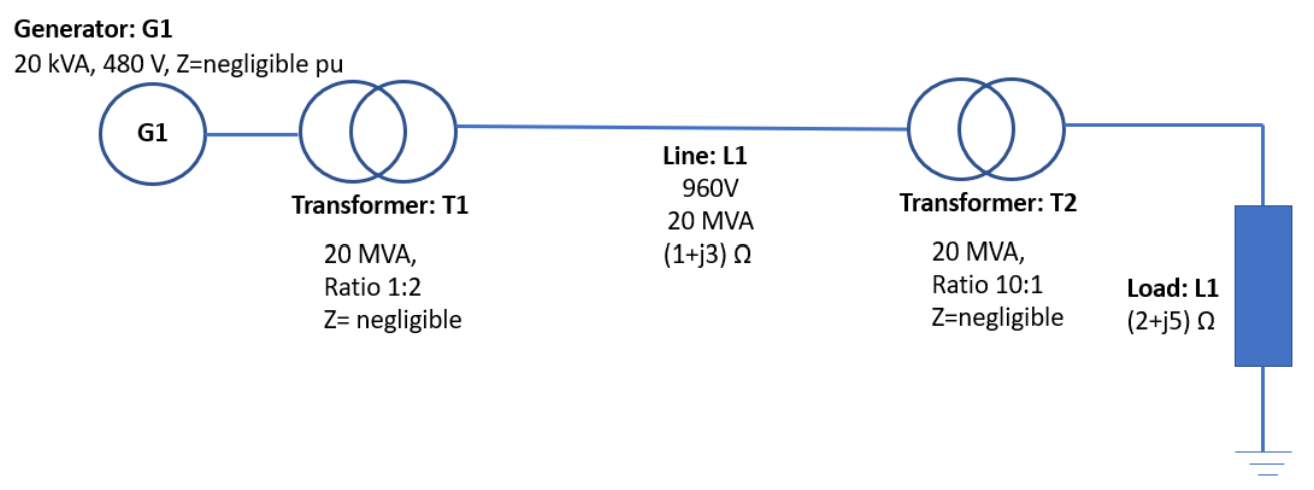
\includegraphics[width = \textwidth]{img/figure150.png}
    \caption{Quiz 3, Question 1. Diagram.}
\end{figure}
G1, T1 and T2 have negligible impedances and can be set to $Z = 0$.

System base (base for generator 1):
\begin{align}
    S_{base,1} & = \SI{20}{kVA}                                                   \\
    V_{base,1} & = \SI{480}{V}                                                    \\
    I_{base,1} & = \frac{20\times 10^3}{\sqrt{3}\times 480} = \SI{24.06}{\ampere} \\
    Z_{base,1} & = \frac{480}{24.06} = \SI{19.95}{\ohm}
\end{align}
Line 1 voltage is \SI{960}{\volt}, hence we recalculate our base values. Let us call this section 2.
\begin{align}
    S_{base,2} & = \SI{20}{kVA}                                                    \\
    V_{base,2} & = \SI{960}{V}                                                     \\
    I_{base,2} & = \frac{20\times 10^3}{\sqrt{3}\times 960} = \SI{12.028}{\ampere} \\
    Z_{base,2} & = \frac{960}{12.028} = \SI{79.812}{\ohm}                          \\
    Z          & = \frac{1+j3}{79.812} = 0.0125 + j0.0376\,\si{pu}
\end{align}
Load 1 voltage is \SI{96}{\volt}, hence we recalculate our base values. Let us call this section 3.
\begin{align}
    S_{base,3} & = \SI{20}{kVA}                                                   \\
    V_{base,3} & = \SI{96}{V}                                                     \\
    I_{base,3} & = \frac{20\times 10^3}{\sqrt{3}\times 96} = \SI{120.28}{\ampere} \\
    Z_{base,3} & = \frac{96}{120.28} = \SI{0.798}{\ohm}                           \\
    Z          & = \frac{2+j5}{0.798} = 2.506+j6.266\,\si{pu}
\end{align}
Total impedance (all in series hence sum real and imaginary parts):
\begin{align}
    Z_t & = 0.0125 + j0.0376 + 2.506 + j6.266 = 2.5185 + j6.3036 \\
    Z_t & = 6.79\angle\SI{68.22}{\degree pu}
\end{align}
Total generator current (pu):
\begin{align}
    I & = \frac{V}{Z} = \frac{1\angle 0}{6.79\angle 68.22}
    I & = 0.147\angle\SI{-68.22}{\degree pu} = \SI{0.28}{pu}
\end{align}
\section{Question 2}
A three-phase short circuit occurs at point F in the system shown below. Calculate the fault level (MVA) and the short circuit fault current (A). Give your answers in pu in polar form.
\begin{figure}[H]
    \centering
    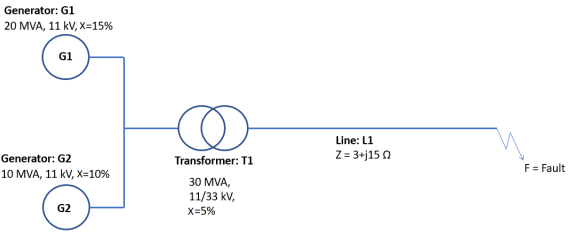
\includegraphics[width = \textwidth]{img/figure154.png}
    \caption{Quiz 3, Question 2. Diagram.}
\end{figure}
System base:
\begin{align}
    S_{base,1} & = \SI{20}{MVA}                                                    \\
    V_{base,1} & = \SI{11}{kV}                                                     \\
    I_{base,1} & = \frac{20\times 10^3}{\sqrt{3}\times 11} = \SI{1049.73}{\ampere} \\
    Z_{base,1} & = \frac{960}{12.028} = \SI{79.812}{\ohm}
\end{align}
Generator 1:
\begin{align}
    S & = \SI{1}{pu}     \\
    V & = \SI{1}{pu}     \\
    X & = j\SI{0.15}{pu}
\end{align}
Generator 2:
\begin{align}
    S & = \SI{0.5}{pu}  \\
    V & = \SI{1}{pu}    \\
    X & = j\SI{0.2}{pu}
\end{align}
Transformer 1:
\begin{align}
    S & = \SI{1.5}{pu}    \\
    V & = 1/3\,\si{pu}    \\
    X & = j\SI{0.033}{pu}
\end{align}
Change of voltage for Line L1 section, hence new base values. Impedance pu:
\begin{align}
    S_{base,2} & = \SI{20}{MVA}                                                   \\
    V_{base,2} & = \SI{33}{kV}                                                    \\
    I_{base,2} & = \frac{20\times 10^3}{\sqrt{3}\times 33} = \SI{349.91}{\ampere} \\
    Z_{base,2} & = \frac{960}{12.028} = \SI{94.31}{\ohm}                          \\
    Z          & = \frac{3+j15}{94.31} = 0.0318+j0.159                            \\
    Z          & = 0.162\angle\SI{78.69}{\degree pu}
\end{align}
Total equivalent impedance for circuit (redraw the SLD with proper impedances and perform reduction calculations for impedances in parallel and series):
\begin{align}
    Z_t & = \frac{j0.15\times j0.2}{j0.15 +j0.2} + j0.033+0.0318+j0.159 \\
    Z_t & = 0.0318 +j0.2777
\end{align}
MVA fault level:
\begin{align}
    MVA_{fault} & = \frac{20}{\sqrt{0.0318^2+0.2777^2}} \\
    MVA_{fault} & = \SI{71.55}{MVA}
\end{align}
Fault current (we use the base voltage at the fault):
\begin{align}
    I_{fault} & = \frac{71.55\times 10^6}{\sqrt{3}\times 33\times 10^3} \\
    I_{fault} & = \SI{1251.8}{\ampere}
\end{align}
\section{Question 3}
In a three-phase star connected load, the following sequence components for phase a were established:
\begin{align}
    V_{a1} & = 0.584+j0 \,\si{pu} \\
    V_{a2} & = 0.584+j0 \,\si{pu} \\
    V_{a0} & = 0 \,\si{pu}
\end{align}
Determine the line voltages $V_{ab}$, $V_{bc}$, $V_{ca}$ in polar form.

`a' matrix to determine phase voltages:
\begin{gather}
    \begin{bmatrix}
        V_a \\
        V_b \\
        V_c
    \end{bmatrix} = \begin{bmatrix}
        1 & 1   & 1   \\
        1 & a^2 & a   \\
        1 & a   & a^2
    \end{bmatrix}\begin{bmatrix}
        0\angle\SI{0}{\degree}     \\
        0.584\angle\SI{0}{\degree} \\
        0.584\angle\SI{0}{\degree}
    \end{bmatrix}
\end{gather}
Hence:
\begin{align}
    V_a & = \left(0\angle\SI{0}{\degree}+0.584\angle\SI{0}{\degree}+0.584\angle\SI{0}{\degree}\right)                                            \\
    V_b & = \left(\left(0\angle\SI{0}{\degree}\right)+a^2\left(0.584\angle\SI{0}{\degree}\right)+a\left(0.584\angle\SI{0}{\degree}\right)\right) \\
    V_b & = \left(a^2 + a\right)\left(0.584\angle\SI{0}{\degree}\right) = 0.584\angle\SI{180}{\degree}                                           \\
    V_c & = \left(\left(0\angle\SI{0}{\degree}\right)+a\left(0.584\angle\SI{0}{\degree}\right)+a^2\left(0.584\angle\SI{0}{\degree}\right)\right) \\
    V_c & = \left(a + a^2\right)\left(0.584\angle\SI{0}{\degree}\right) = 0.584\angle\SI{180}{\degree}
\end{align}
Line to line voltages:
\begin{align}
    V_{ab} & = V_a - V_b = \left(1.168\angle\SI{0}{\degree}\right) - \left(0.584\angle\SI{180}{\degree}\right) = 1.752\angle\SI{0}{\degree} \\
    V_{bc} & = V_b - V_c = \left(0.584\angle\SI{180}{\degree}\right) - \left(0.584\angle\SI{180}{\degree}\right) = 0\angle\SI{0}{\degree}   \\
    V_{ca} & = V_c - V_a = \left(0.584\angle\SI{0}{\degree}\right) - \left(1.168\angle\SI{0}{\degree}\right) = 1.752\angle\SI{180}{\degree}
\end{align}
\section{Question 5}
Consider all types of balanced and unbalanced faults that can be experienced in an electrical power system. Hence, undertake a study of investigation to determine their severity. List the most severe to least severe.

Faults in descending order of severity:
\begin{enumerate}
    \item Three phase balanced
    \item Double line to ground
    \item Line to line
    \item Single line to ground
    \item Double phase open circuit
    \item Single phase open circuit
\end{enumerate}